% Latex template: mahmoud.s.fahmy@students.kasralainy.edu.eg
% For more details: https://www.sharelatex.com/learn/Beamer

\documentclass{beamer}					% Document class
\geometry{papersize={15cm,10cm}}

\setbeamertemplate{footline}[text line]{%
  \parbox{\linewidth}{\vspace*{-8pt}\hfill\hfill\insertpagenumber}}
\setbeamertemplate{navigation symbols}{}

\usepackage[english]{babel}				% Set language
\usepackage[utf8x]{inputenc}			% Set encoding

\mode<presentation>						% Set options
{
  \usetheme{default}					% Set theme
  \usecolortheme{default} 				% Set colors
  \usefonttheme{default}  				% Set font theme
  \setbeamertemplate{caption}[numbered]	% Set caption to be numbered
}

% Uncomment this to have the outline at the beginning of each section highlighted.
%\AtBeginSection[]
%{
%  \begin{frame}{Outline}
%    \tableofcontents[currentsection]
%  \end{frame}
\usepackage{graphicx}					% For including figures
\usepackage{booktabs}					% For table rules
\usepackage{hyperref}	
\usepackage{tikz-network}				% For cross-referencing
\usepackage[absolute,overlay]{textpos}
\usepackage{bm}
\usepackage[font=small,labelfont=bf]{caption}				% For cross-referencing
\usepackage{comment}
\usepackage{braket}

\title{Advancing super resolution microscopy for quantitative in-vivo imaging of chromatin nanodomains}	% Presentation title
\author{Clayton W. Seitz}								% Presentation author
\date{\today}									% Today's date	

\setbeamertemplate{footline}{
    \hbox{%
    \begin{beamercolorbox}[wd=\paperwidth,ht=3ex,dp=1.5ex,leftskip=2ex,rightskip=2ex]{page footer}%
        \usebeamerfont{title in head/foot}%
        \insertshorttitle \hfill
            \insertsection \hfill
        \insertframenumber{} / \inserttotalframenumber
    \end{beamercolorbox}}%
}

\AtBeginSection[]{
  \begin{frame}
  \vfill
  \centering
  \begin{beamercolorbox}[sep=8pt,center,shadow=true,rounded=true]{title}
    \usebeamerfont{title}\insertsectionhead\par%
  \end{beamercolorbox}
  \vfill
  \end{frame}
}

\begin{document}

% Title page
% This page includes the informations defined earlier including title, author/s, affiliation/s and the date
\begin{frame}
  \titlepage
\end{frame}

\begin{frame}{Outline}
    \tableofcontents
\end{frame}



% The following is the most frequently used slide types in beamer
% The slide structure is as follows:
%
%\begin{frame}{<slide-title>}
%	<content>
%\end{frame}

\section{Introduction to fluorescence nanoscopy}

\begin{frame}{Fluorescence microscopy and the diffraction limit}

\begin{textblock*}{9cm}(2.5cm,1.25cm)
Minimal resolvable distance $d \sim \lambda$
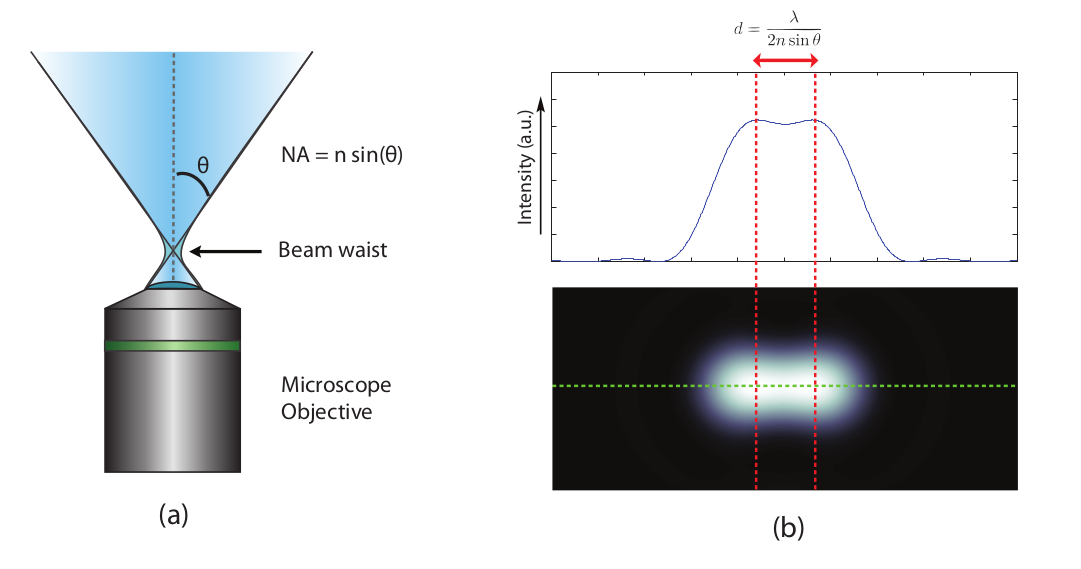
\includegraphics[width=10cm]{media/Limit}
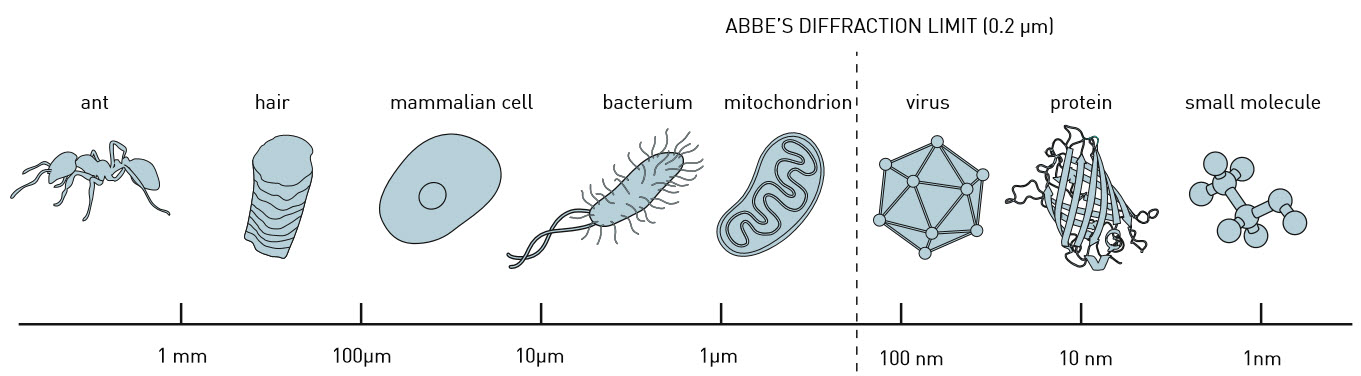
\includegraphics[width=10cm]{media/Scale}
\end{textblock*}

\end{frame}

\begin{frame}{Stochastic optical reconstruction microscopy (STORM)}
\begin{textblock*}{9cm}(0.5cm,1.0cm)
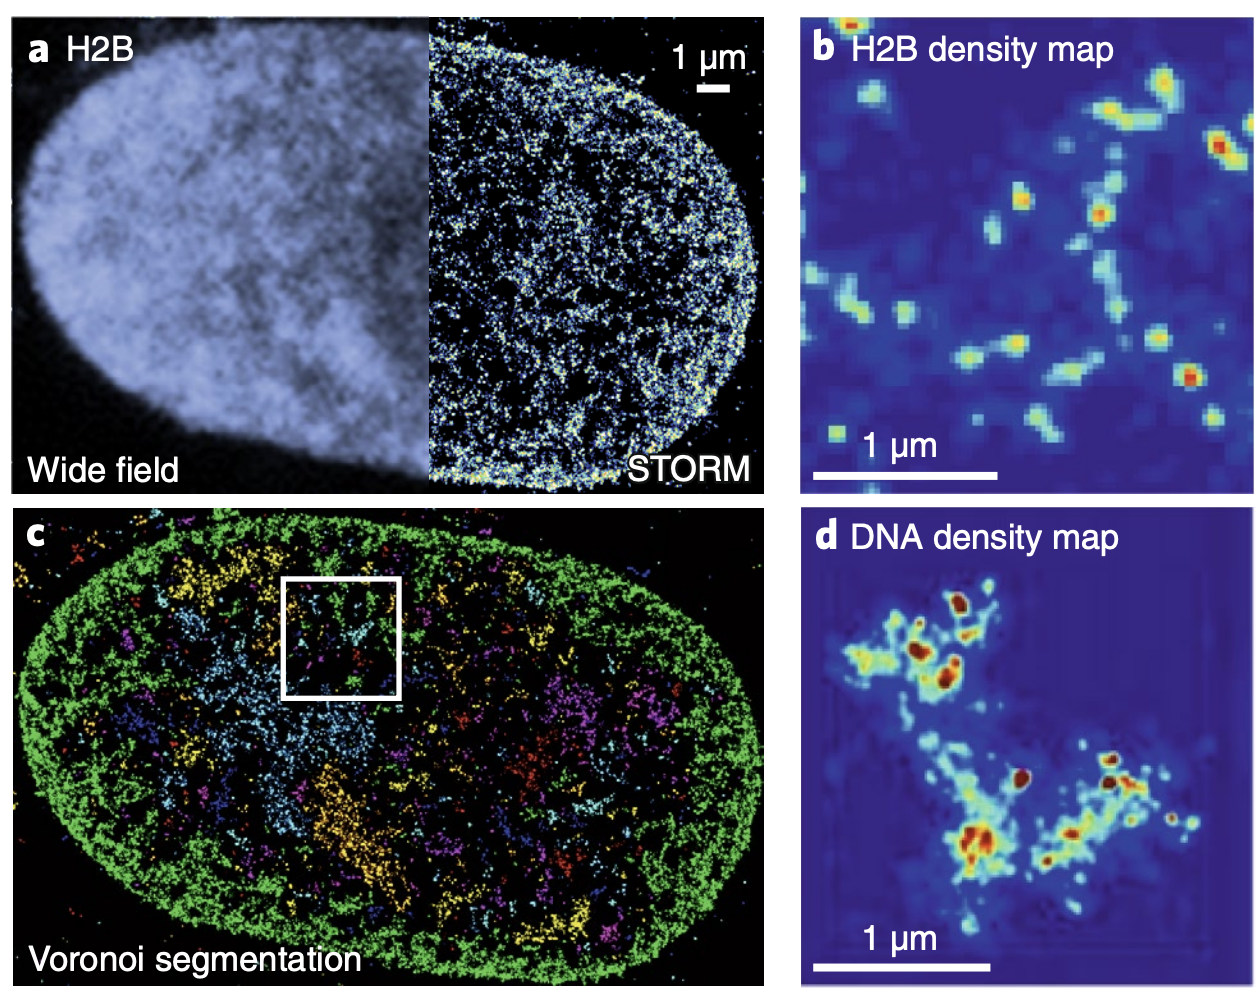
\includegraphics[width=9cm]{media/STORM.png}
Lakadamyali, M. et al. Nature Methods \textbf{17}, (2020).
\end{textblock*}
\begin{textblock*}{3.5cm}(10.0cm,1.1cm)
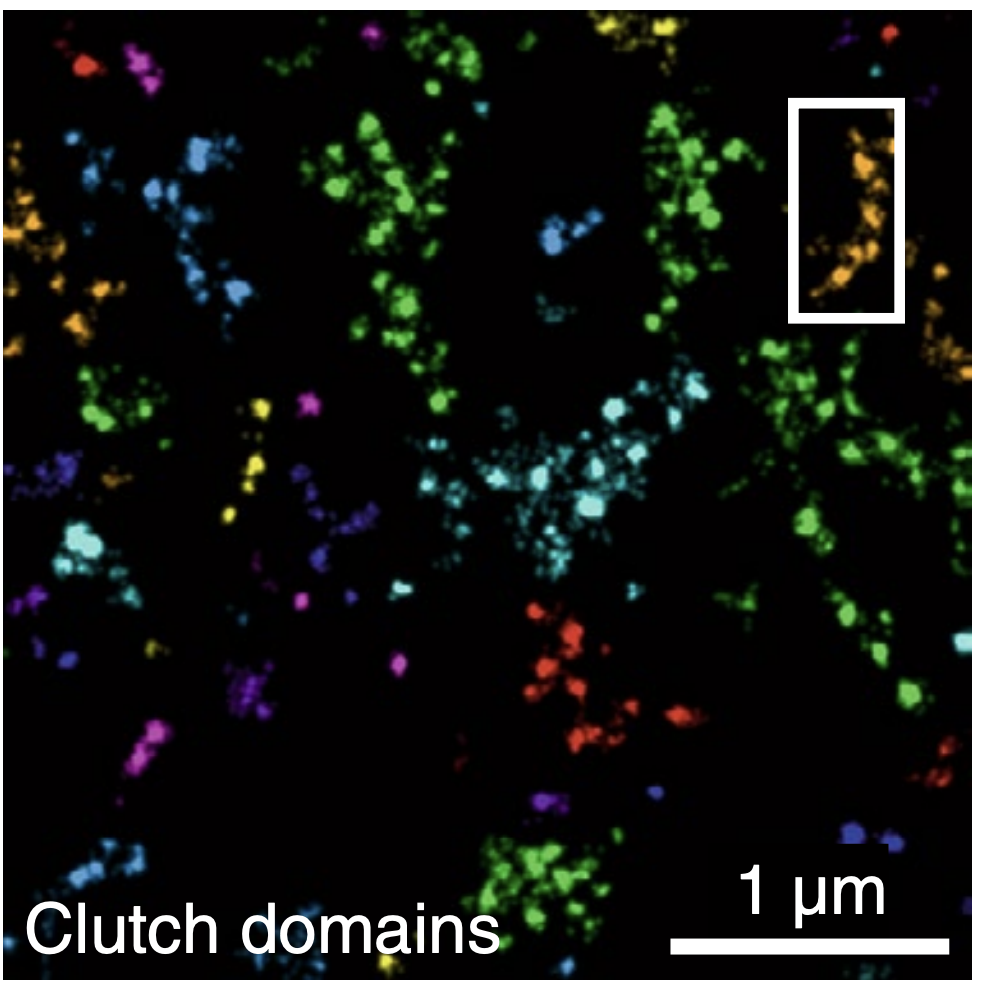
\includegraphics[width=3.5cm]{media/ClutchDomains.png}
\end{textblock*}
\begin{textblock*}{4.5cm}(10.0cm,5.0cm)
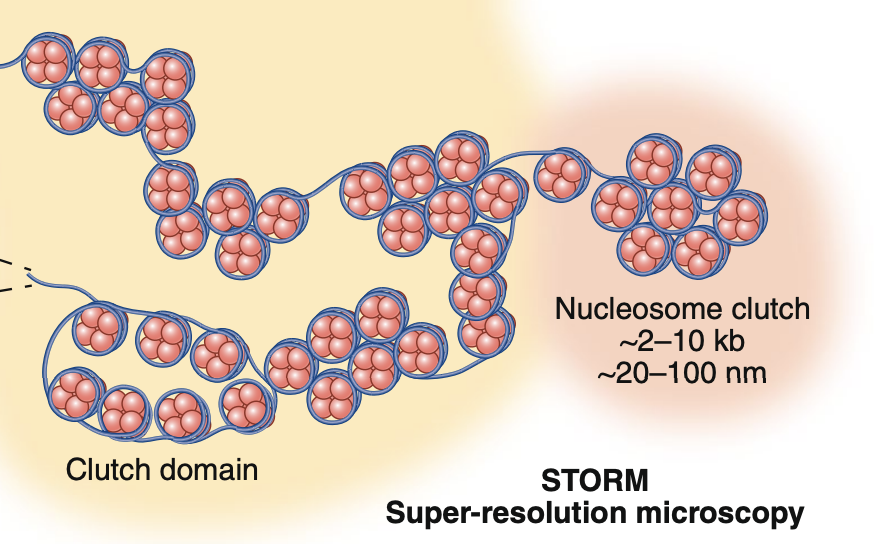
\includegraphics[width=4.5cm]{media/ClutchCartoon.png}
\end{textblock*}
\end{frame}

\begin{frame}{Stochastic optical reconstruction microscopy (STORM)}
\begin{textblock*}{13cm}(1.0cm,1.5cm)
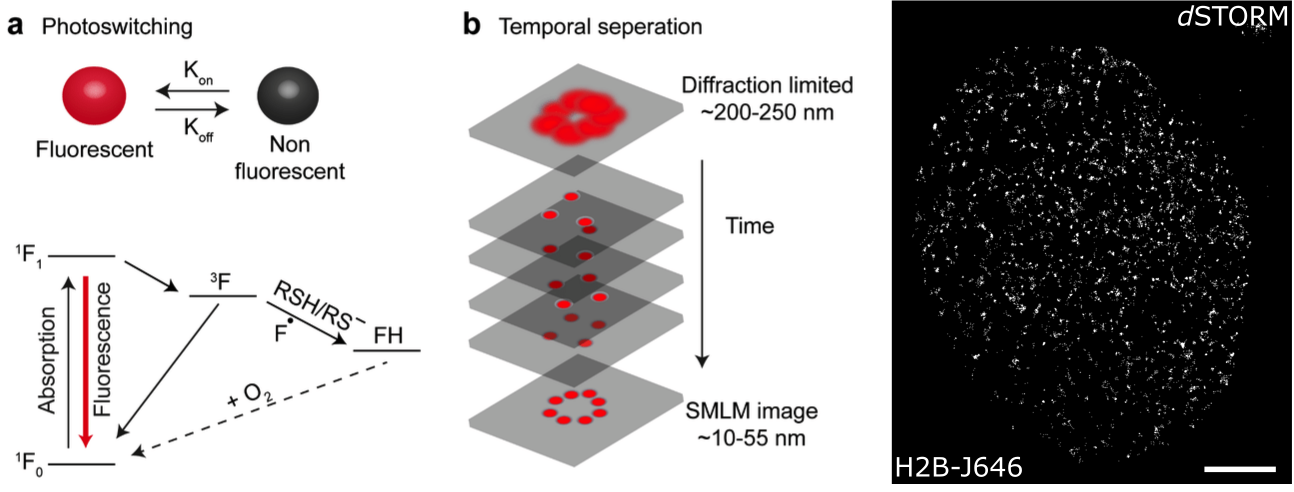
\includegraphics[width=\textwidth]{media/Intro.png}
\end{textblock*}
\begin{textblock*}{\textwidth}(1.0cm,7.5cm)
\begin{itemize}
\item Single molecule localization microscopy (SMLM) techniques are diffraction-unlimited
\item Photoswitching enables resolution of emitters below the diffraction limit
\end{itemize}
\end{textblock*}
\end{frame}


\begin{frame}{Applications of single molecule localization microscopy}
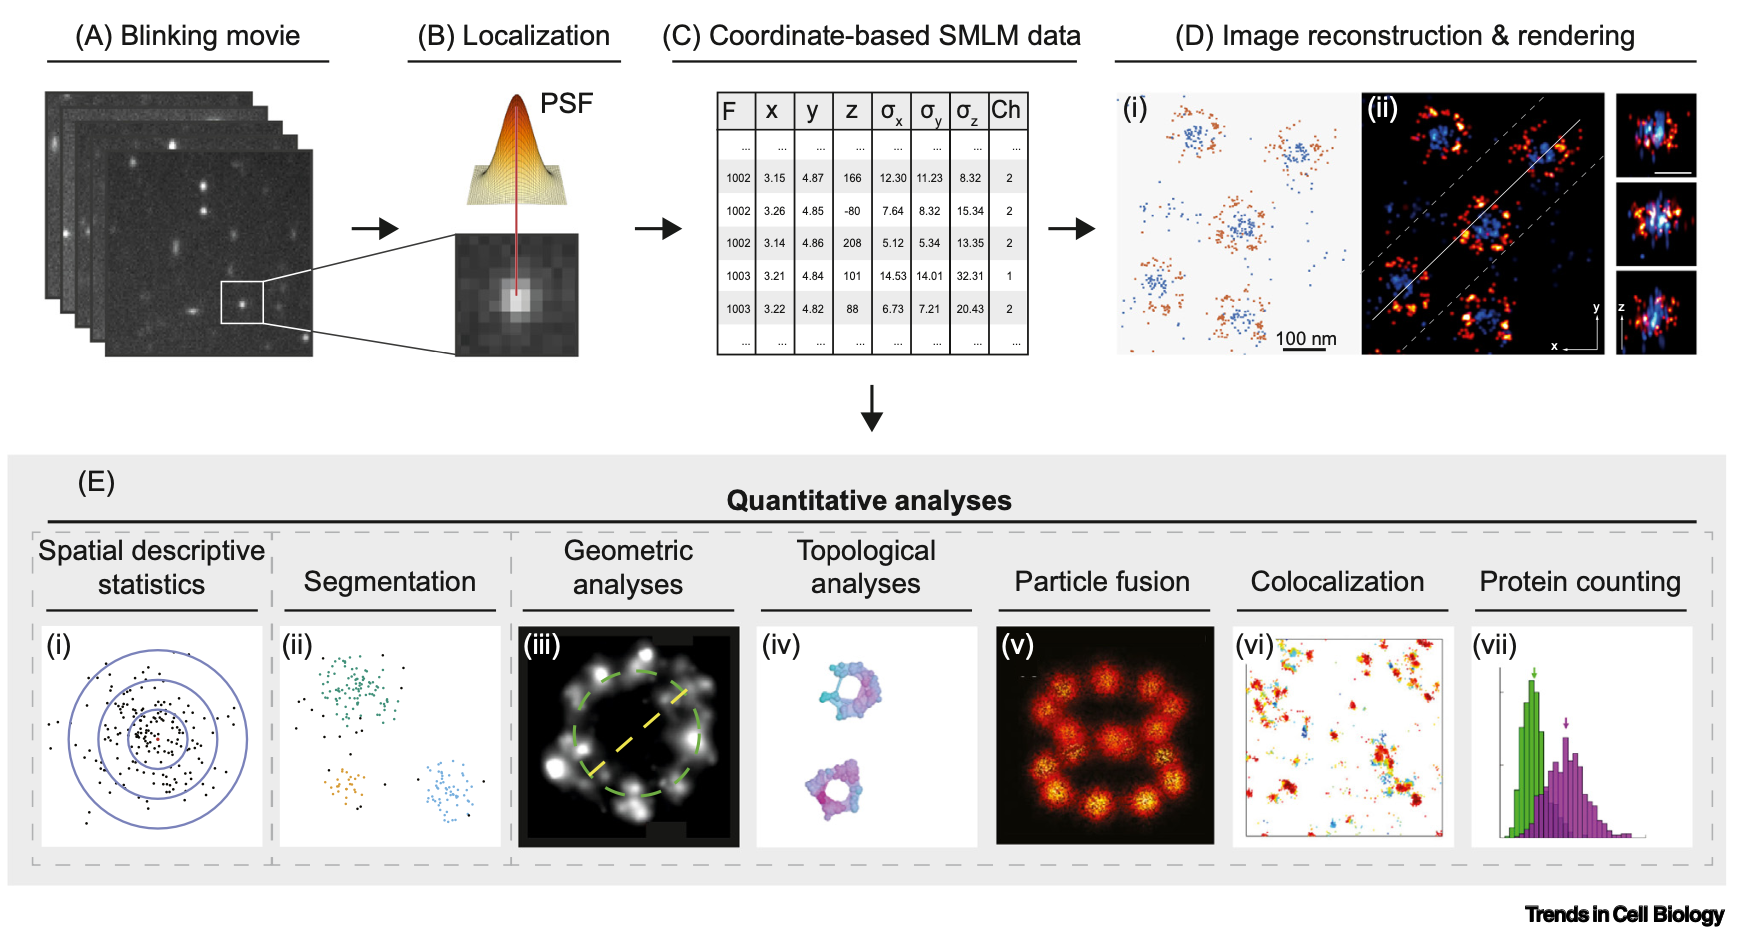
\includegraphics[width=\textwidth]{media/Apps.png}
Wu et al. Trends in Cell Biology. \textbf{30} (2020)
\end{frame}


\begin{comment}
\begin{frame}
\frametitle{Super resolution with photoswitching of rhodamines}

\begin{figure}
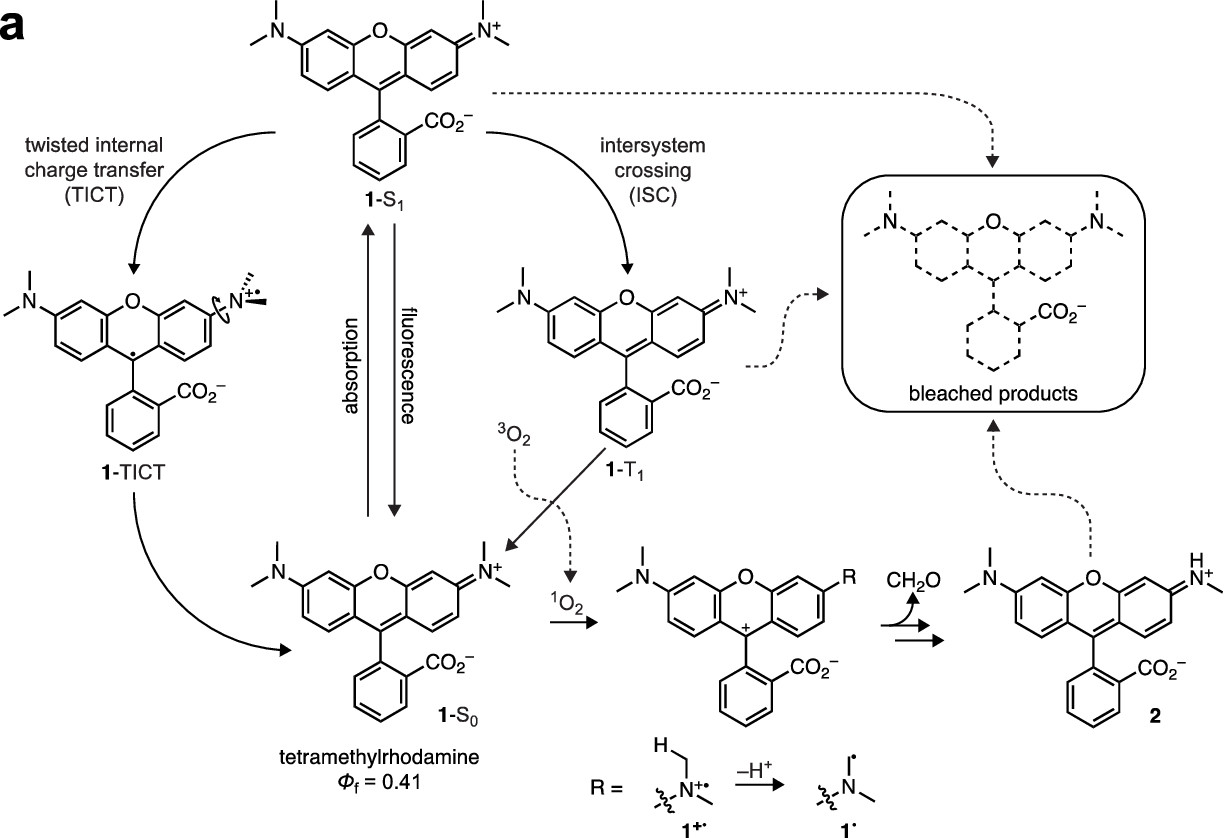
\includegraphics[width=10cm]{media/Rhodamines.png}
\end{figure}
\begin{itemize}
\item  Reduction of the T1 state yields a dark, long-lived, and stable radical state
\end{itemize}
\end{frame}
\end{comment}

\begin{comment}
\begin{frame}
\frametitle{Direct stochastic optical reconstruction microscopy}

\begin{figure}
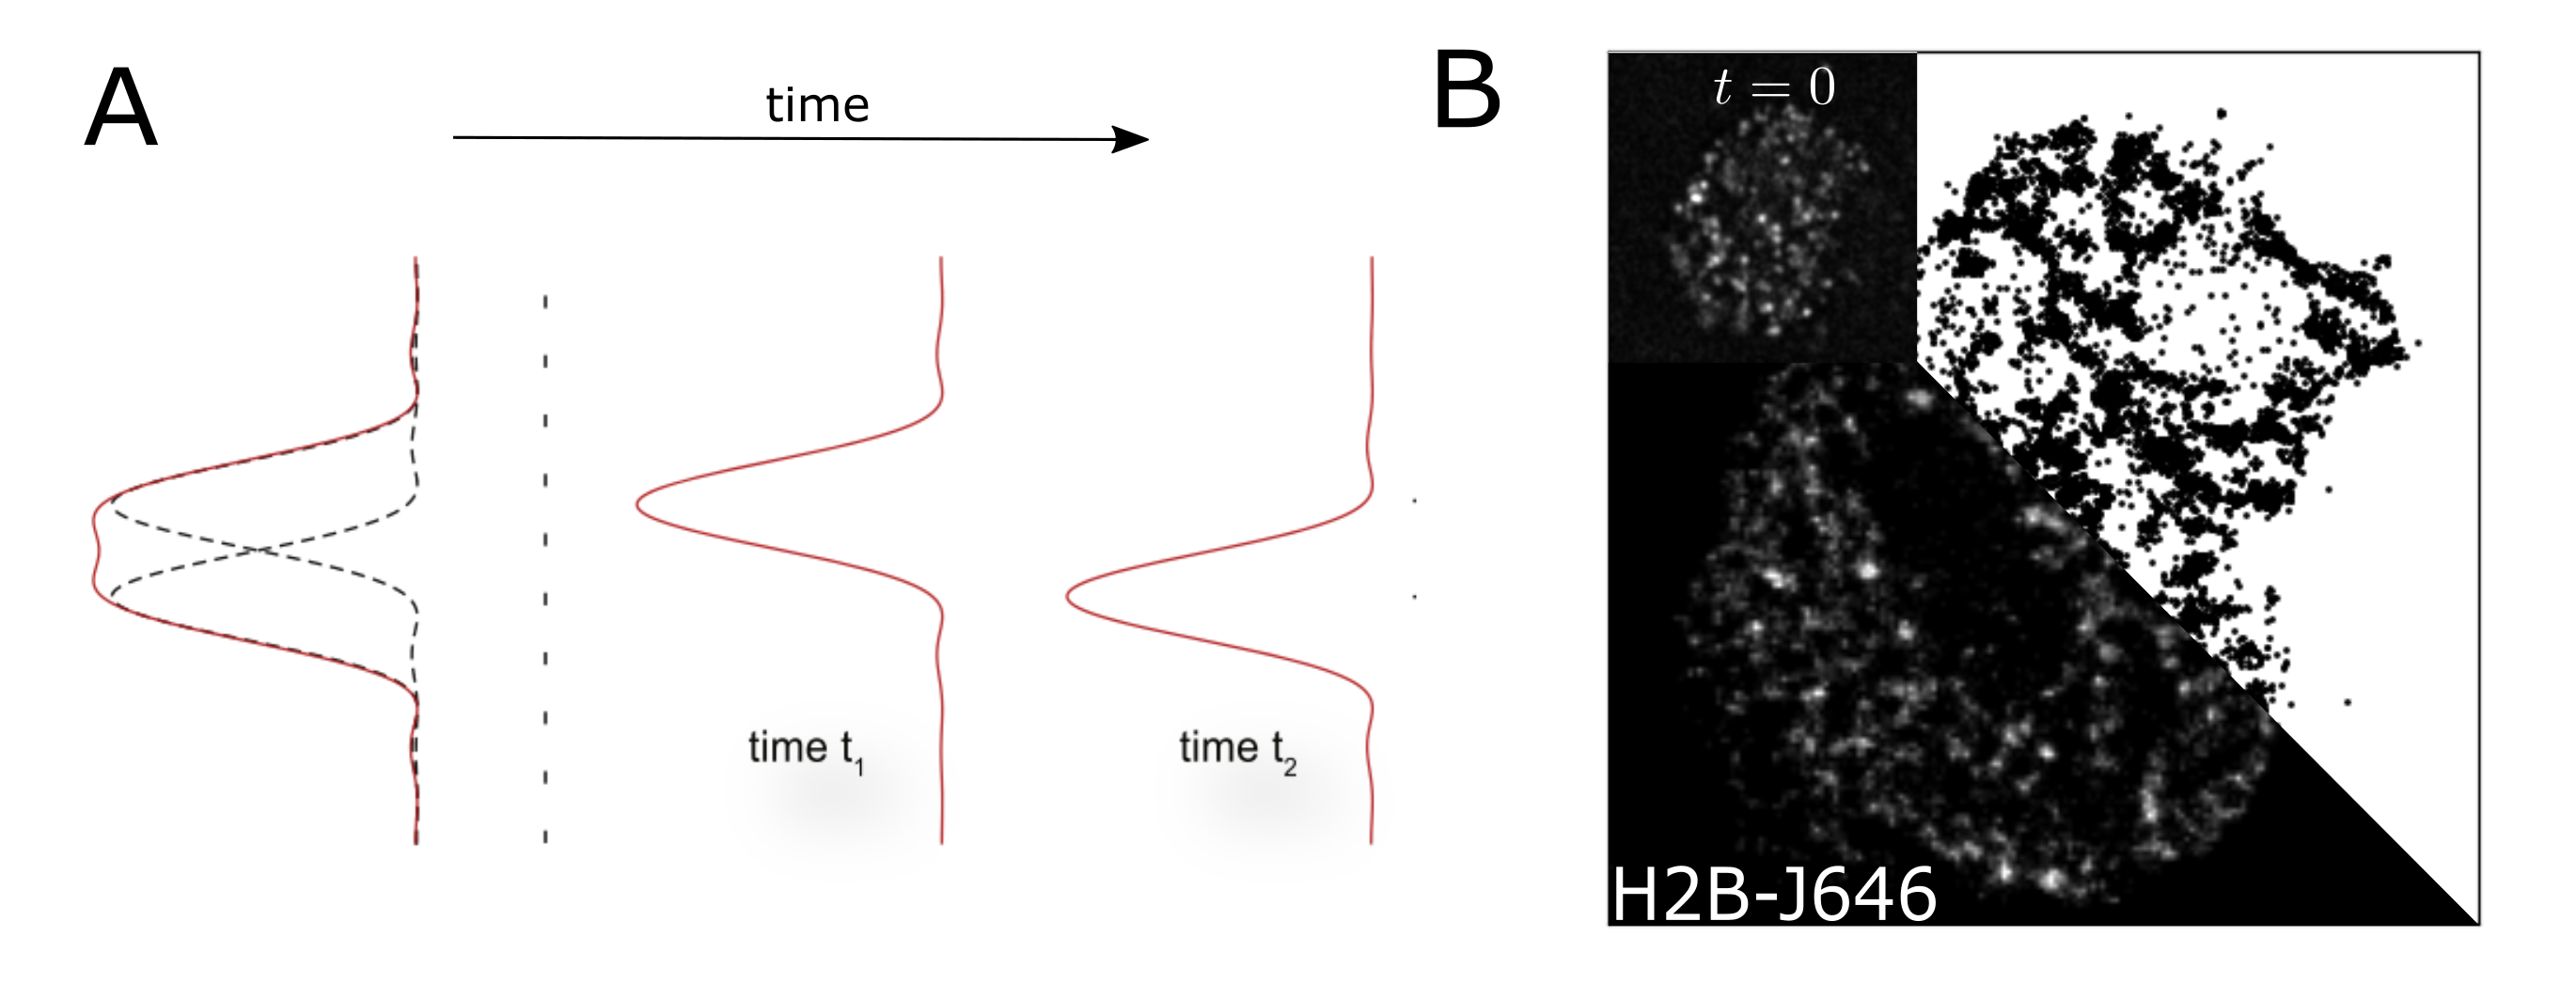
\includegraphics[width=13cm]{media/Concept.png}
\end{figure}

\begin{itemize}
\item Photoswitching enables resolution of emitters in time rather than space
\item Presents a tradeoff between spatial and temporal resolution
\end{itemize}

\end{frame}
\end{comment}


\section{Enhanced nanoscopy with deep generative models}

\begin{frame}{Localization of isolated fluorescent emitters}

Modeling the point spread function permits sub-pixel localization 

\begin{textblock*}{8cm}(6.5cm,2.0cm)
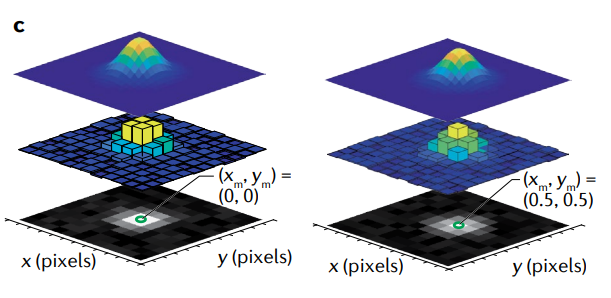
\includegraphics[width=\textwidth]{media/Model.png}
\end{textblock*}

\begin{textblock*}{2cm}(1cm,2.0cm)
\begin{align*}
\mu_{k} &= i_{0}\int\int O(u,v)dudv\\
i_{0} &= g_{k}\textcolor{red}{\eta} \textcolor{cyan}{N_{0}}\textcolor{blue}{\Delta} 
\\
g_{k} &- \mathrm{pixel\; gain}\\
\textcolor{red}{\eta} &- \mathrm{quantum\; efficiency}\\
\textcolor{cyan}{N_{0}} &- \mathrm{photon\; emission\; rate}\\
\textcolor{blue}{\Delta} &- \mathrm{exposure\; time}
\end{align*}
\end{textblock*}

\vspace{2in}

Assume $N_{0}$ is constant over $\textcolor{blue}{\Delta}$ (homogeneous Poisson)

\begin{equation*}
\theta^{*} = \underset{\theta}{\mathrm{argmax}}\prod_{k}P(\bold{x}_{k}|\theta)= \underset{\theta}{\mathrm{argmin}}-\sum_{k}\log P(\bold{x}_{k}|\theta)
\end{equation*}

\end{frame}

\begin{frame}{How to pack more localizations in a single frame?}
Cast localization as \emph{image restoration}
\vspace{1cm}
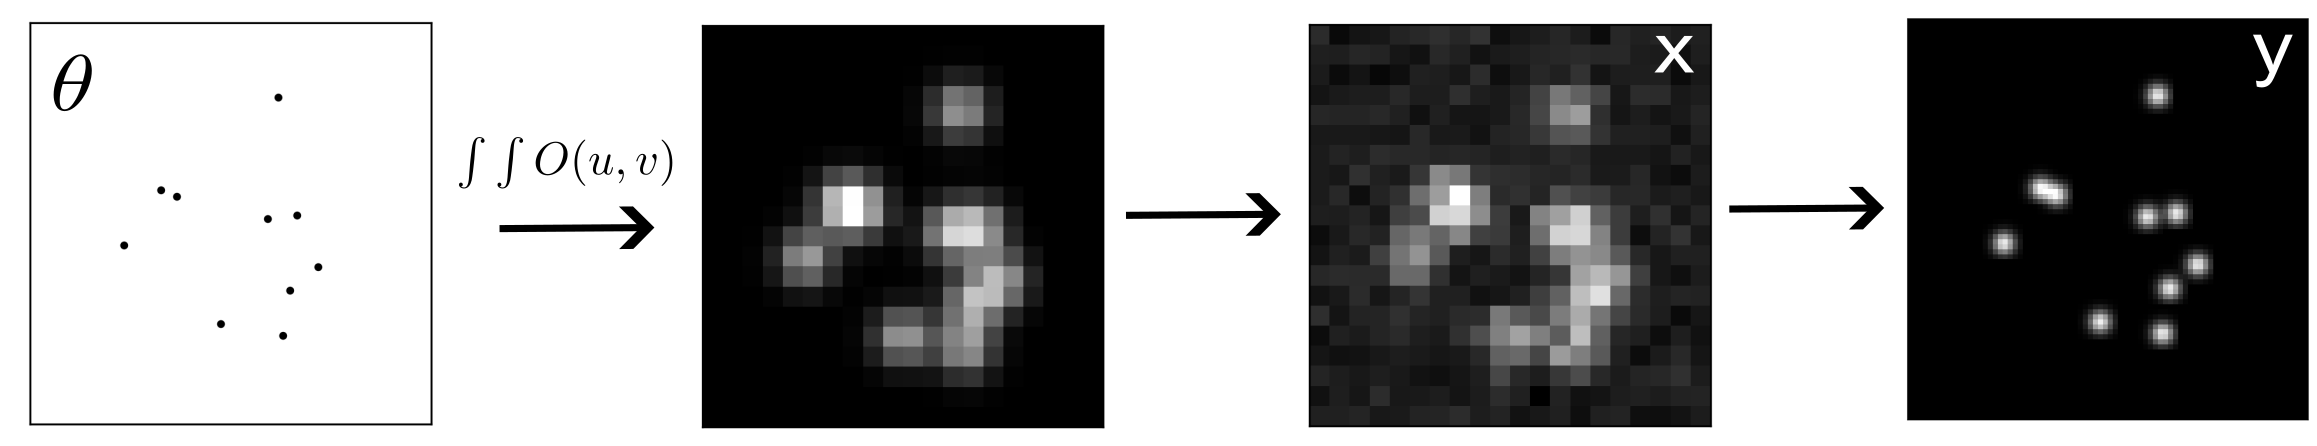
\includegraphics[width=\textwidth]{media/Generation.png}\\
Seitz et al. Under Review. (2024) \\
\vspace{1cm}
\begin{itemize}
\item Would like to estimate a high-resolution $\bold{y}$ from low-resolution $\bold{x}$, but it is many to one
\item Must then model a \emph{distribution} over $\bold{y}$ i.e., $p(\bold{y}|\bold{x})$
\item How to model a distribution over images?
\end{itemize}
\end{frame}


\begin{frame}{Bayesian image restoration with diffusion models}
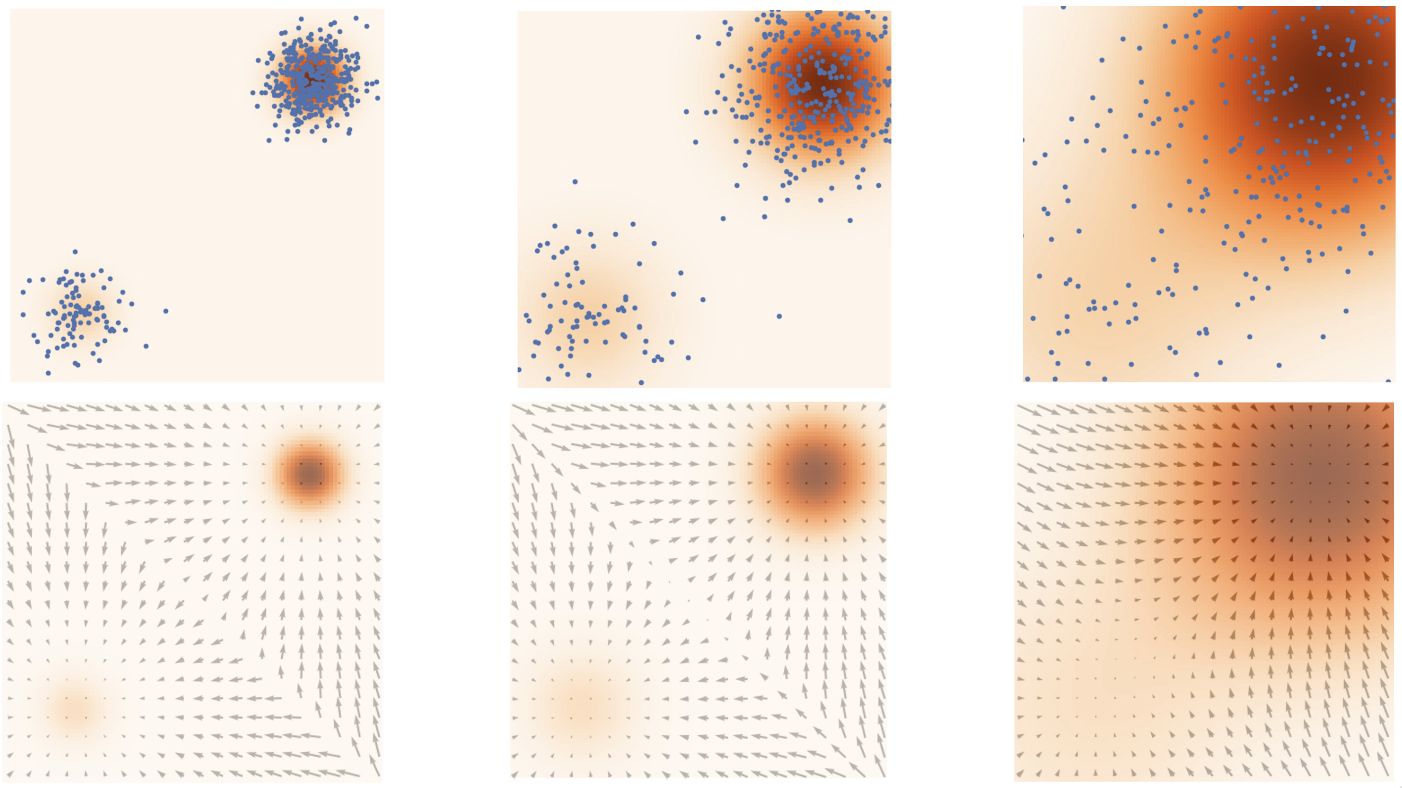
\includegraphics[width=\textwidth]{media/Scores.png}
\end{frame}

\begin{frame}

\begin{align}
-\log p(\bold{y}_{0}) &\leq -\mathbb{E}_{q(\bold{y}_{1:T}|\bold{y}_{0})} \log \left(\frac{p_{\psi}(\bold{y}_{1:T},\bold{y}_{0})}{q(\bold{y}_{1:T}|\bold{y}_{0})}\right) \\
&=  D_{KL}(q(\bold{y}_{T}|\bold{y}_{0}) || p(\bold{y}_{T})) + \mathbb{E}_{q(\bold{y}_{1}|\bold{y}_{0})} \log p(\bold{y}_{0}|\bold{y}_{1}) + \mathcal{L}_{\psi}
\end{align}

\end{frame}



\section{Super-resolution of nucleosome nanodomains \textit{in-vivo}}

\begin{frame}{Hierarchical structure of chromatin}

\begin{textblock*}{10cm}(3.0cm,1.25cm)
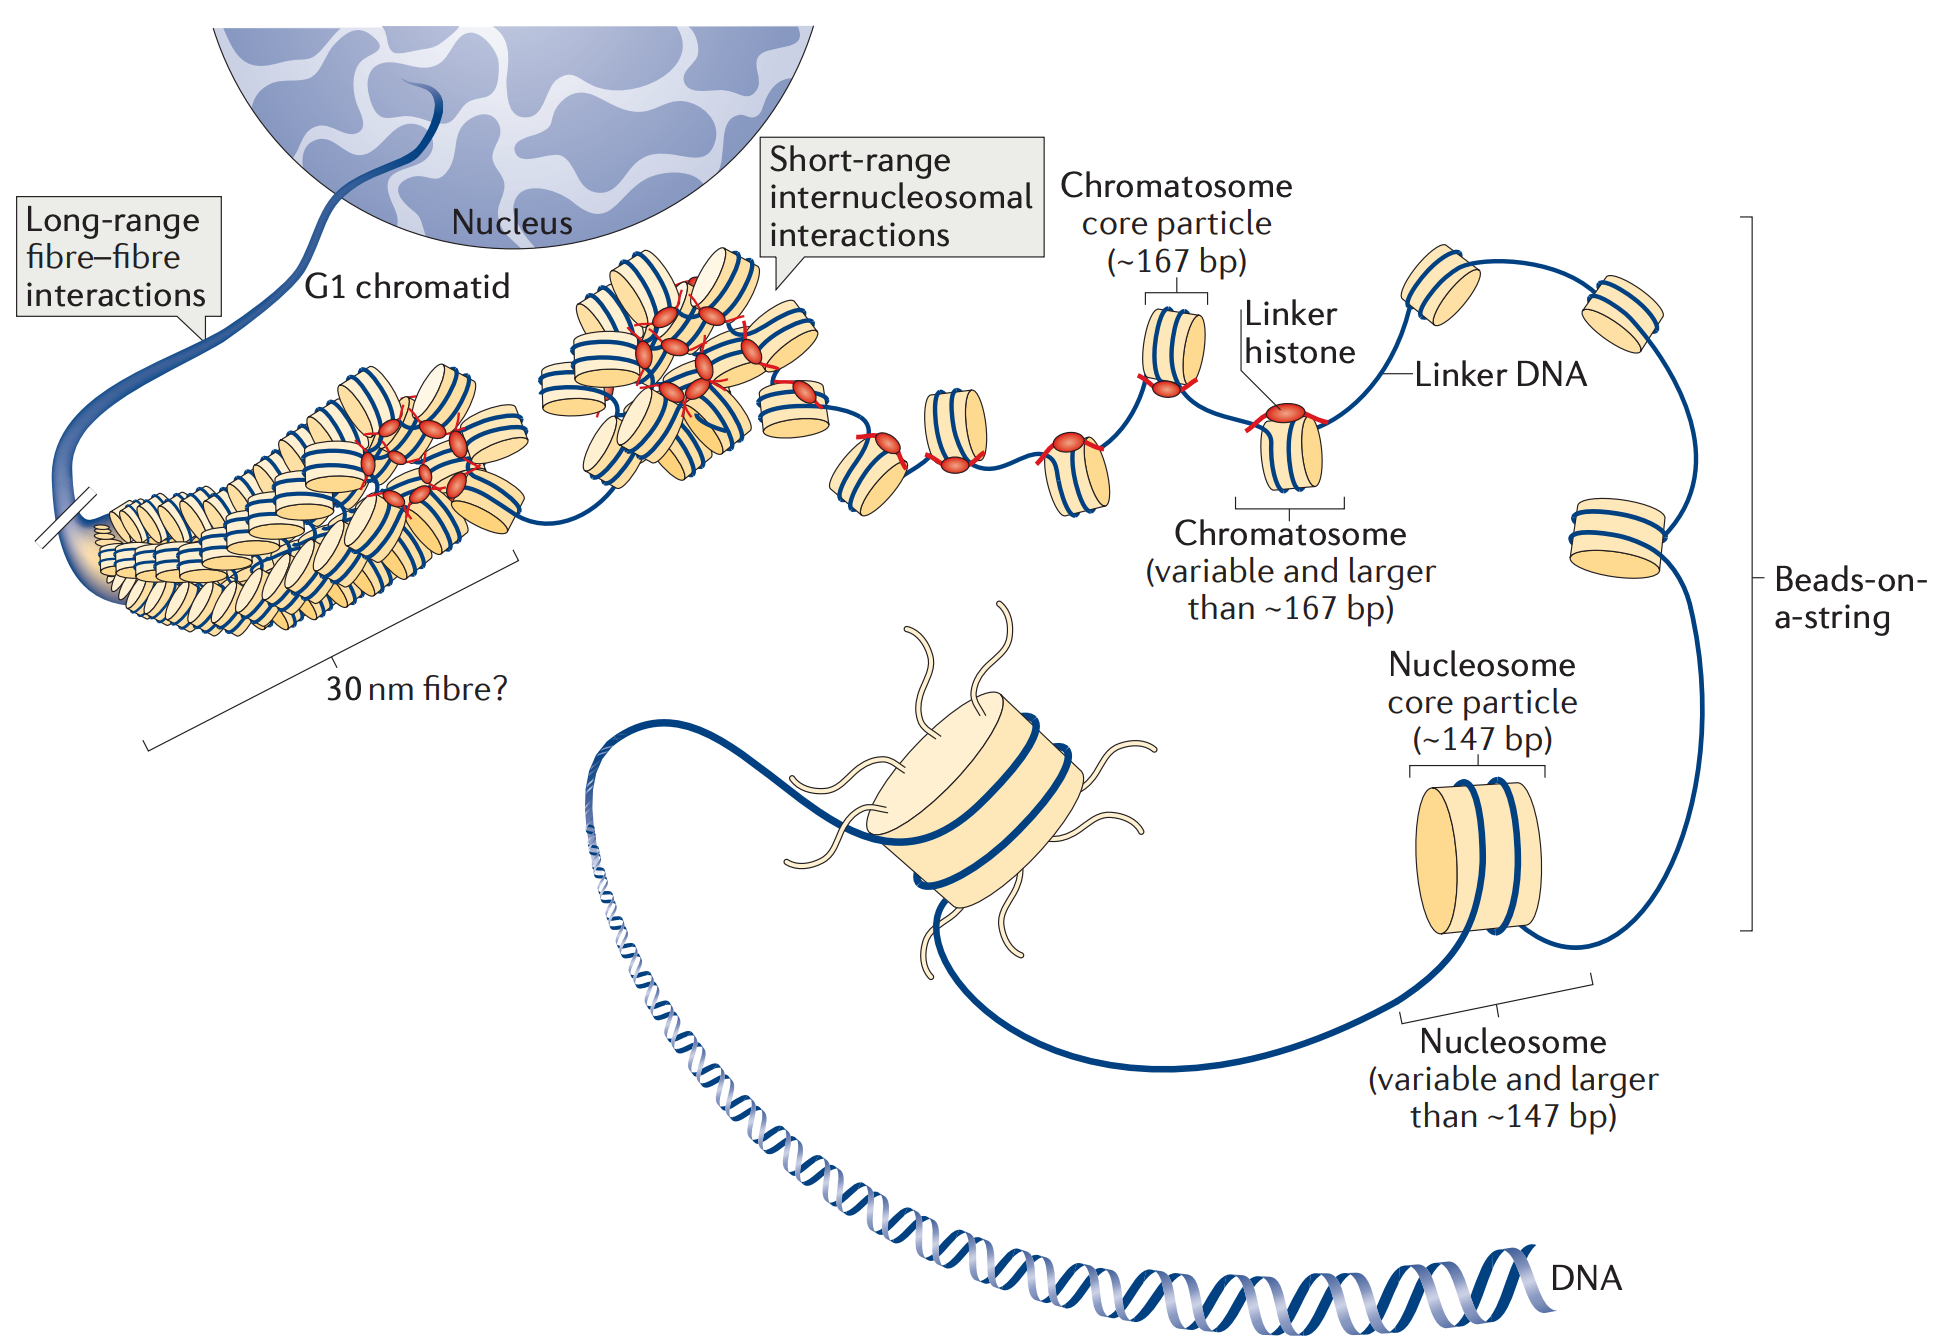
\includegraphics[width=10cm]{media/Chromatin}
\\
\vspace{0.4cm}
Fyodorov, D. et al. Nat Rev Mol Cell Biol \textbf{19}, (2018).
\end{textblock*}

\end{frame}

\begin{frame}{Bromodomain protein 4 (BRD4) binds acetylated chromatin}

\begin{textblock*}{5cm}(2.0cm,1.75cm)
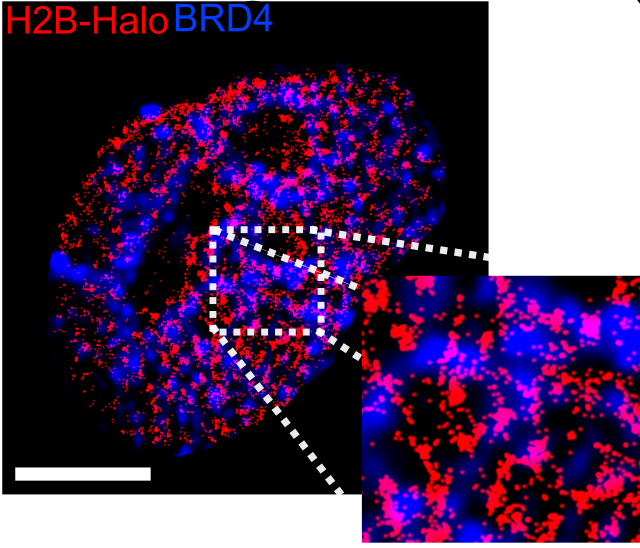
\includegraphics[width=5cm]{media/TwoColor}
\end{textblock*}

\begin{textblock*}{5cm}(7.75cm,1.25cm)
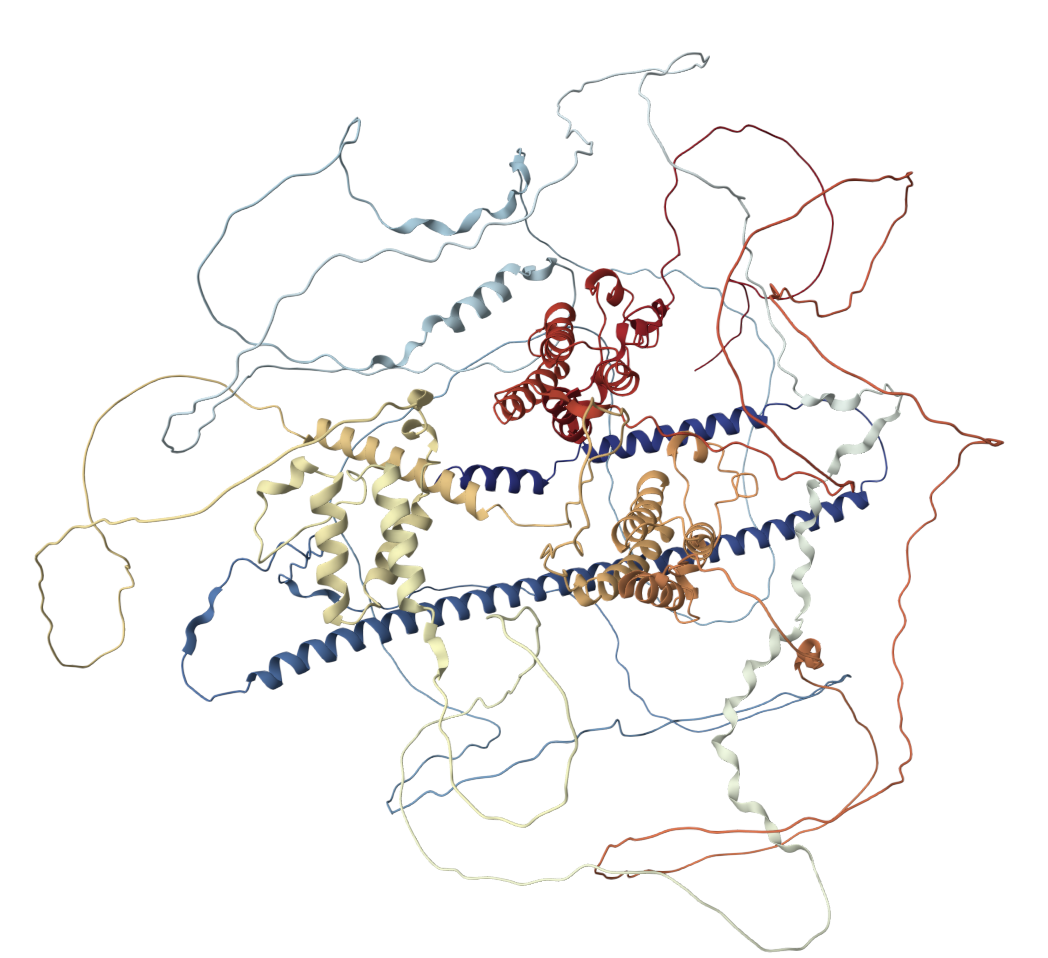
\includegraphics[width=5cm]{media/BRD4-Structure}
\end{textblock*}

\begin{textblock*}{10cm}(2.0cm,7.0cm)
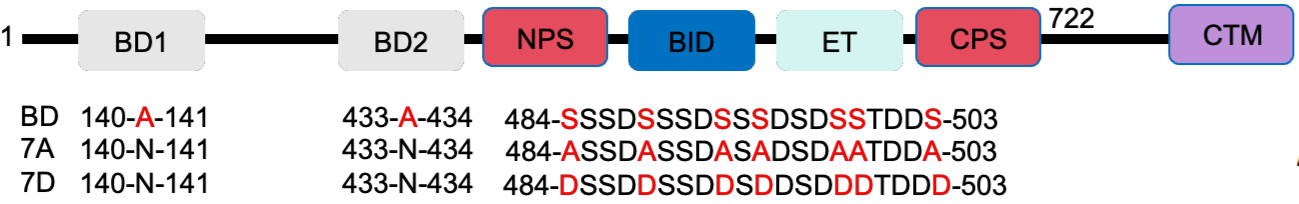
\includegraphics[width=10cm]{media/Mutations}
\end{textblock*}

\end{frame}


\begin{frame}
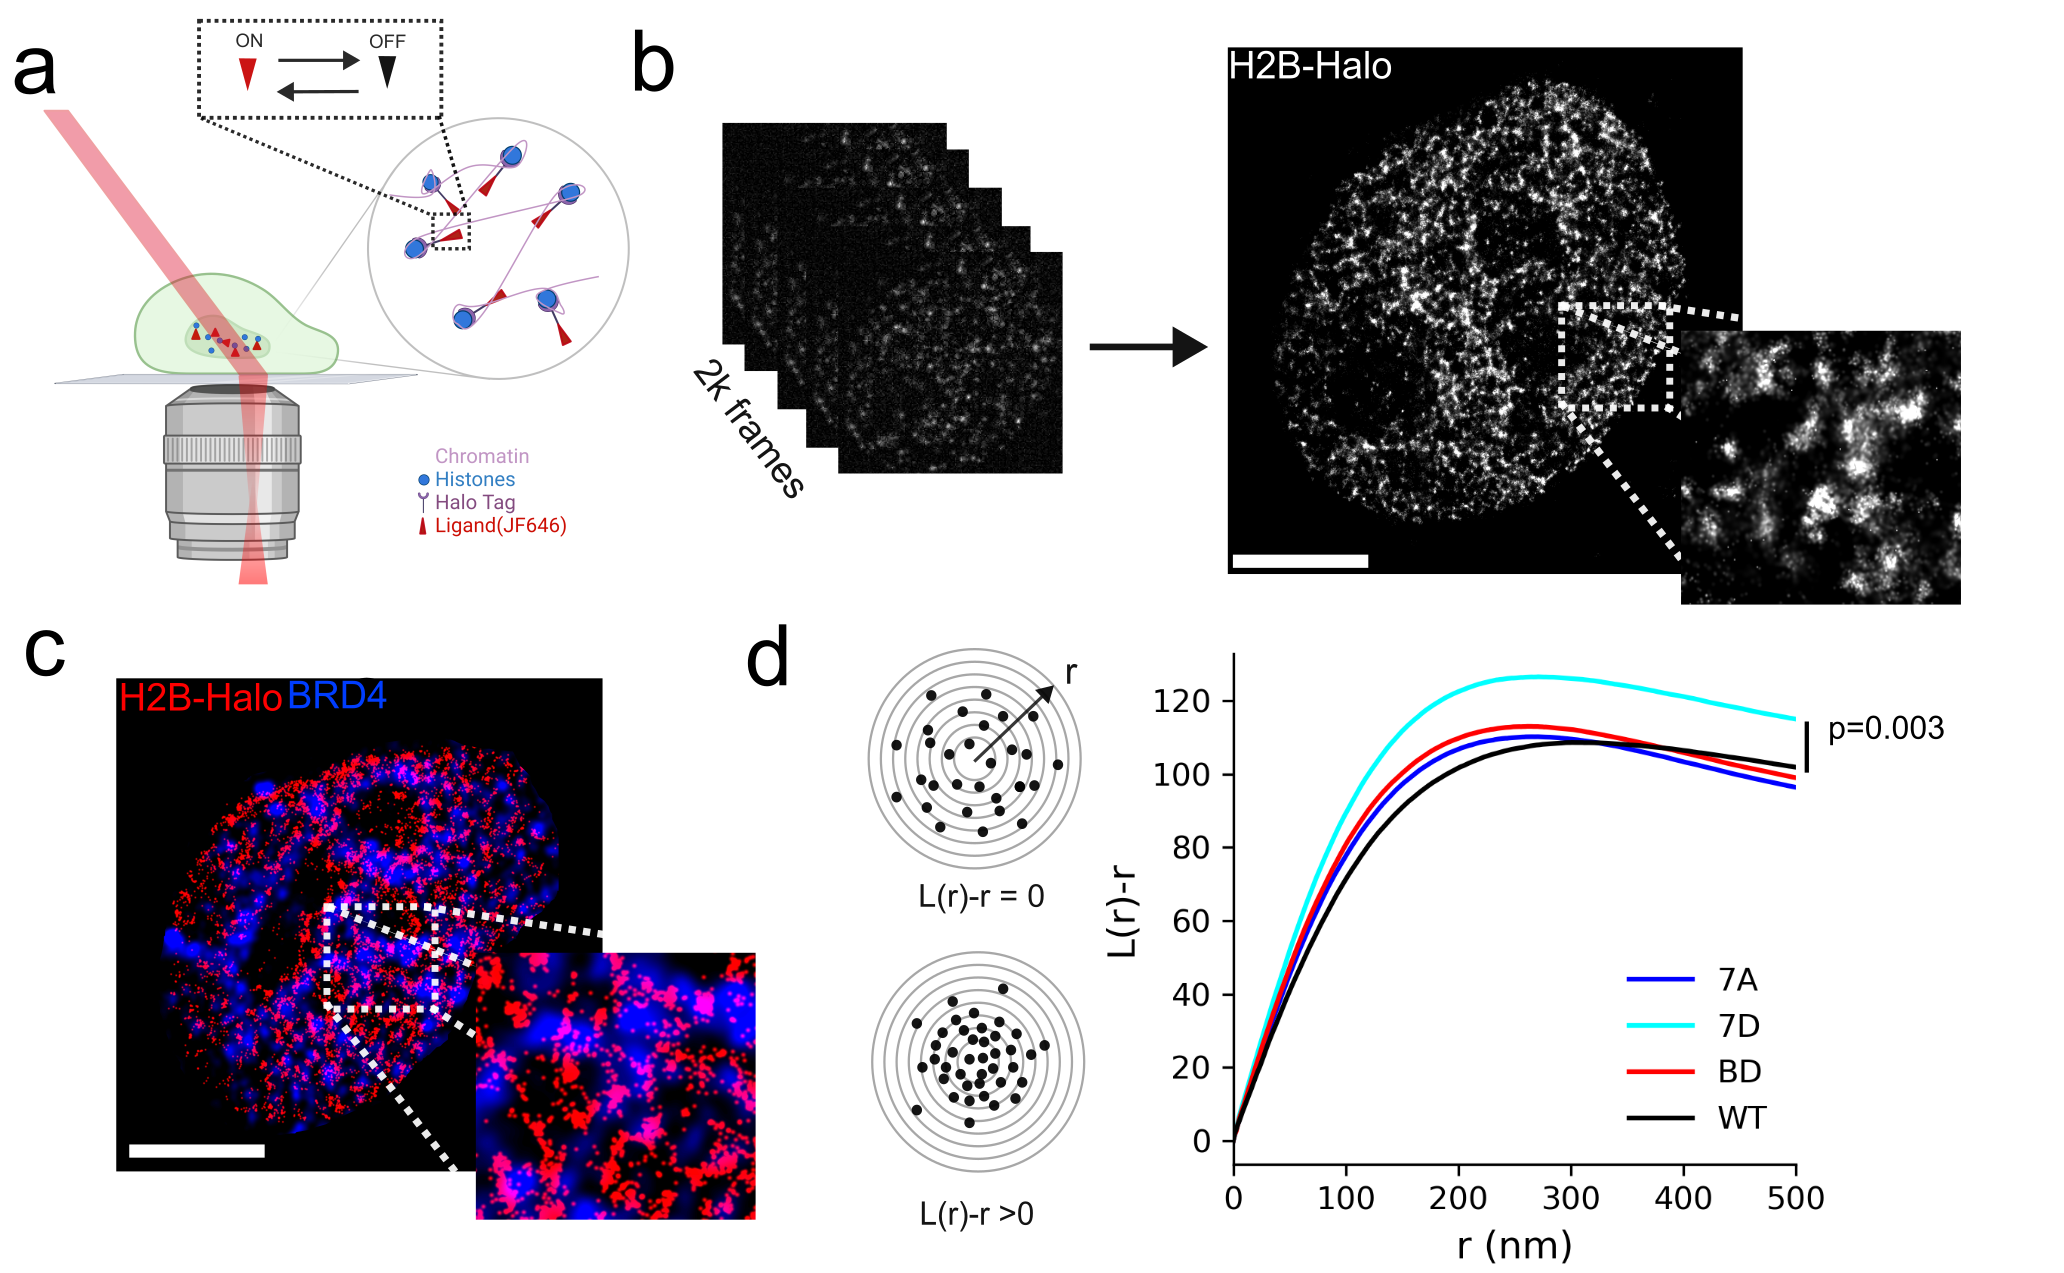
\includegraphics[width=12cm]{media/BRD4-STORM}
\\
Seitz et al. Under Review. (2020)
\end{frame}

\begin{frame}
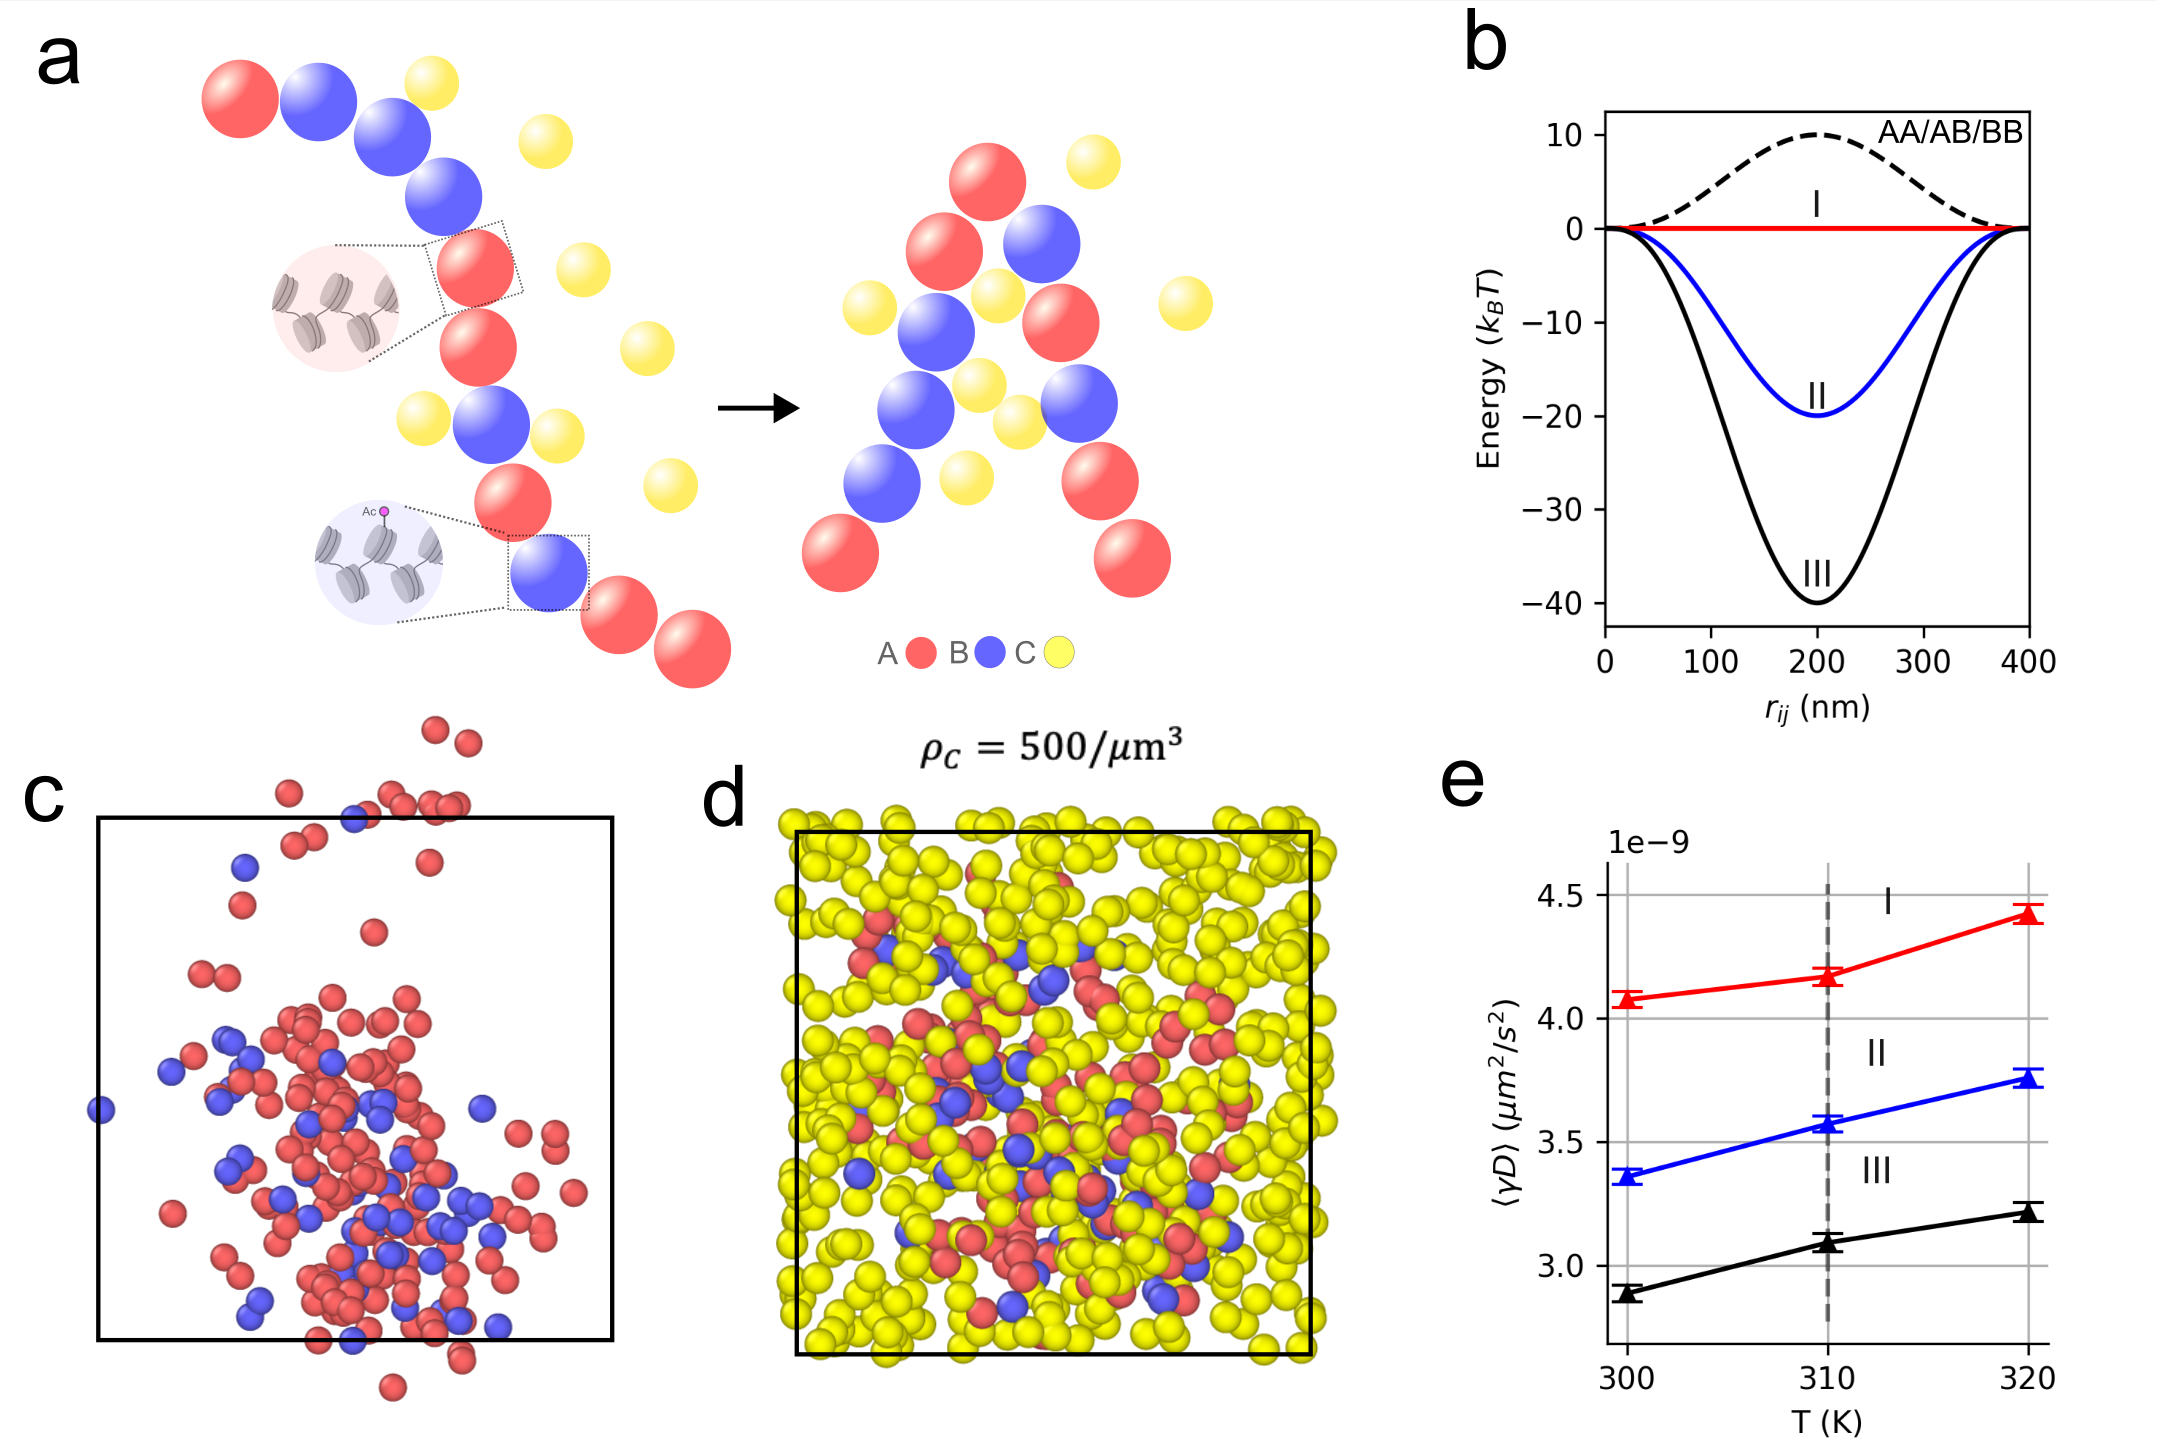
\includegraphics[width=12cm]{media/MD}
\\
Seitz et al. Under Review. (2020)
\end{frame}

\begin{frame}
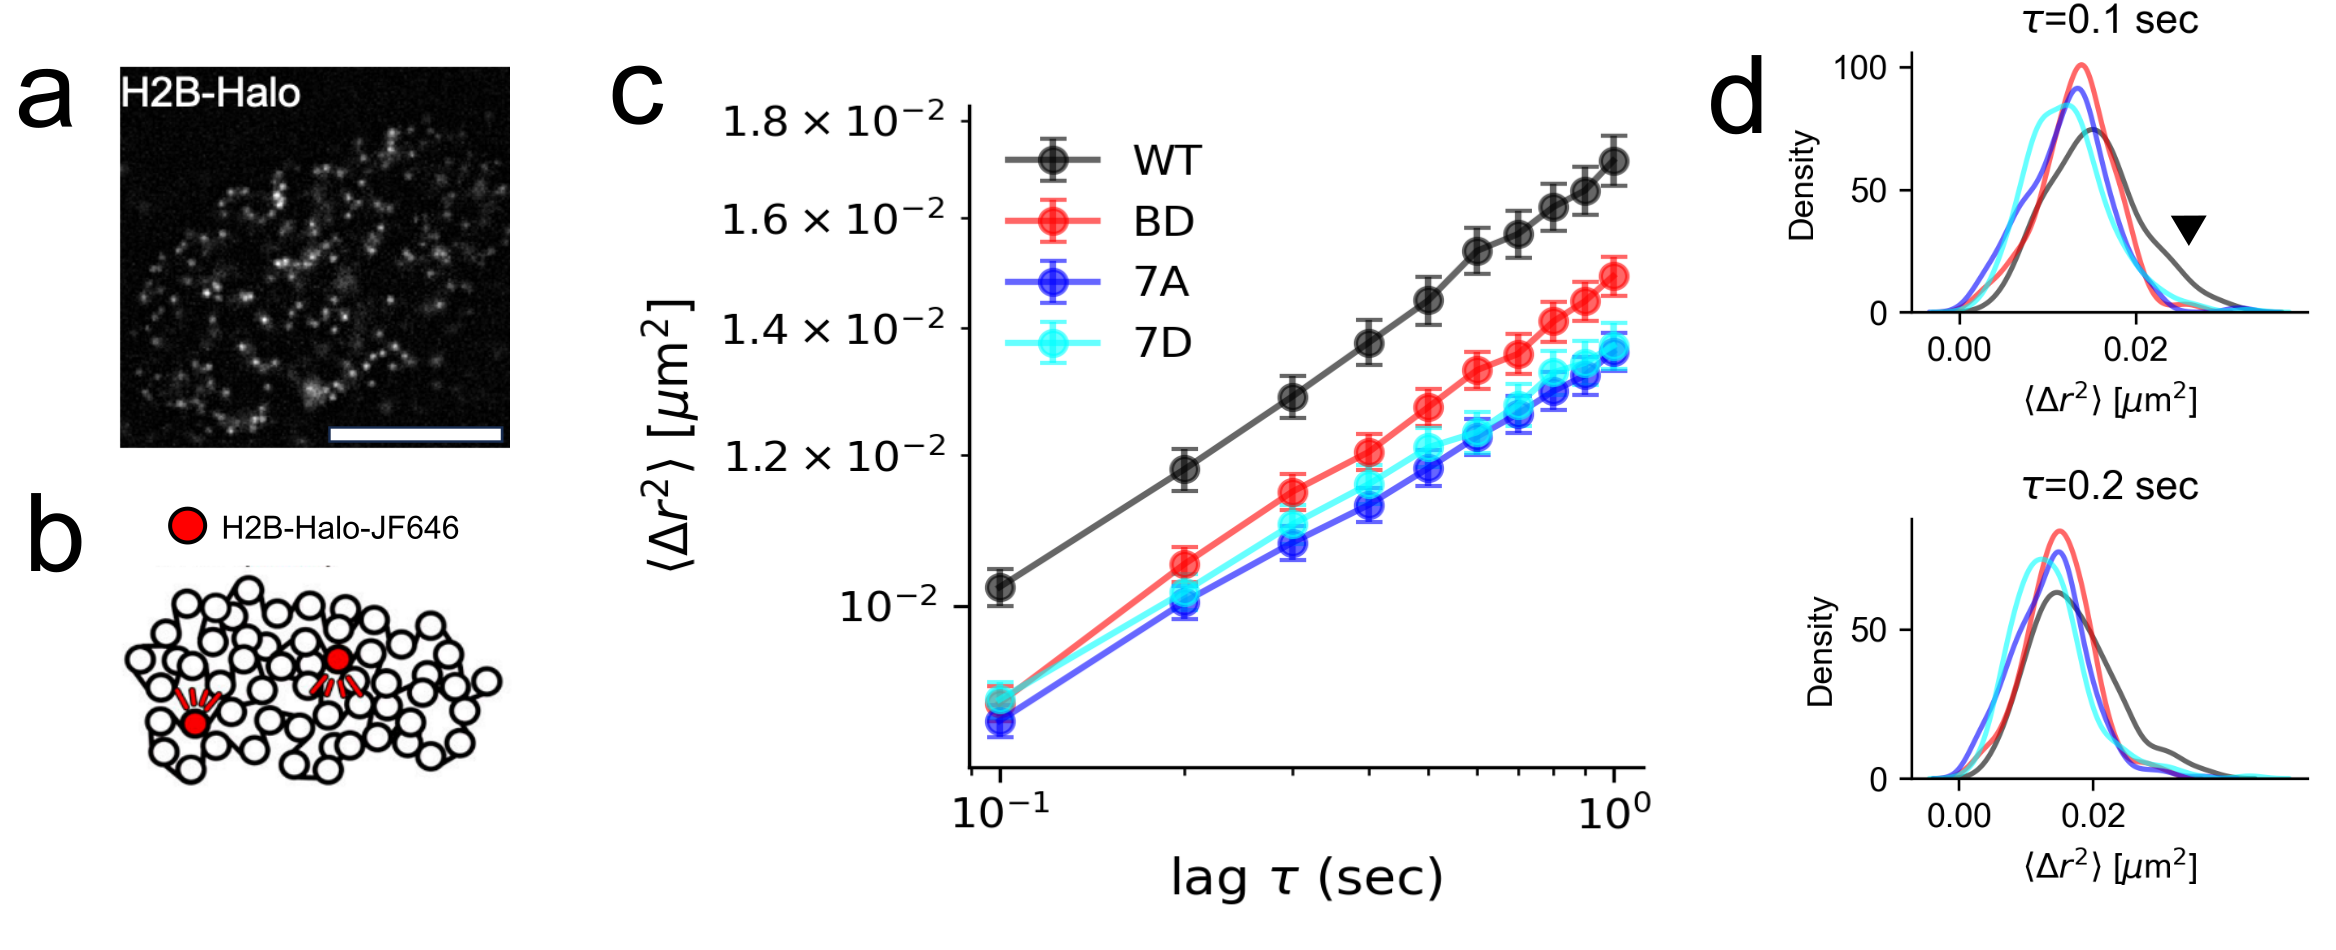
\includegraphics[width=12cm]{media/MSD}
\\
Seitz et al. Under Review. (2024)
\end{frame}


\begin{frame}{Recent Publications}

\begin{itemize}
\item Maelle Locatelli\textsuperscript{\textdagger}, Josh Lawrimore\textsuperscript{\textdagger}, Hua Lin\textsuperscript{\textdagger}, Sarvath Sanaullah, \textbf{Clayton Seitz}, ..., Pierre-Alexandre Vidi. \textit{DNA damage reduces heterogeneity and coherence of chromatin motions}. PNAS. July 2022\\
\vspace{0.1in}
\item Mengdi Zhang, \textbf{Clayton Seitz}, Garrick Chang, Fadil Iqbal, Hua Lin, and Jing Liu \textit{A guide for single-particle chromatin tracking in live cell nuclei}. Cell Biology International. January 2022.\\
\vspace{0.1in}
\item Wenting Wu, Farooq Syed, Edward Simpson, Chih-Chun Lee, Jing Liu, Garrick Chang, Chuanpeng Dong, \textbf{Clayton Seitz}, ..., Carmella Evans-Molina; \textit{Impact of Proinflammatory Cytokines on Alternative Splicing Patterns in Human Islets}. Diabetes. January 2022
\end{itemize}
\end{frame}

\begin{frame}{Acknowledgements}
\begin{textblock*}{14cm}(0.5cm,1.5cm)
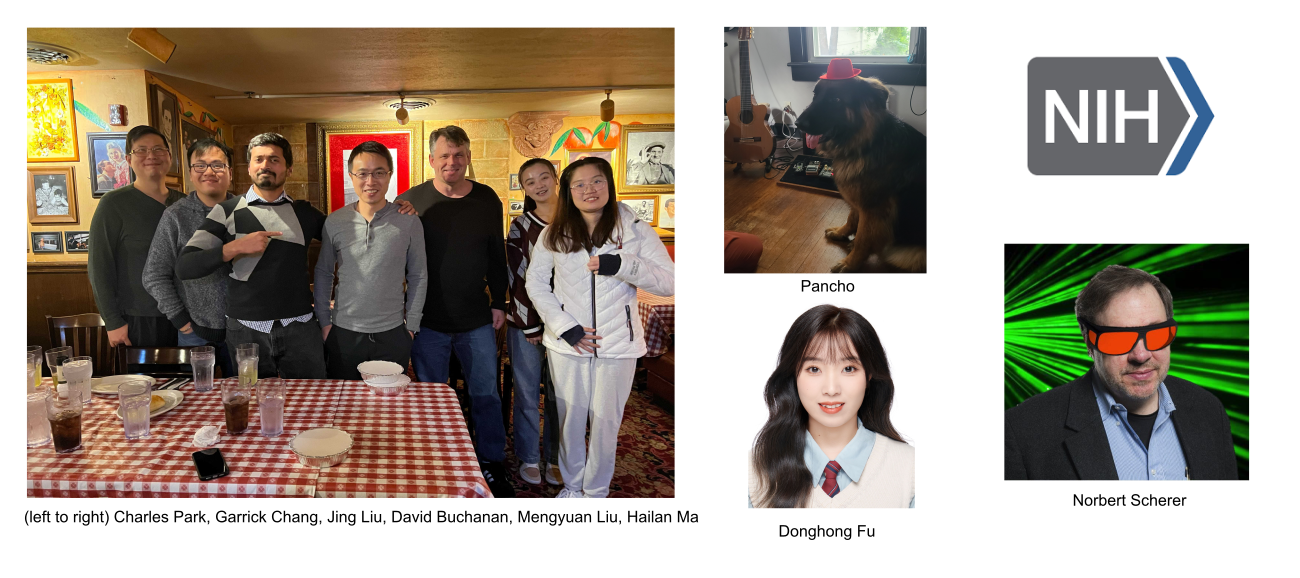
\includegraphics[width=14cm]{media/Lab.png}
\end{textblock*}

\begin{textblock*}{14cm}(0.5cm,8.5cm)
Thank you!
\end{textblock*}

\end{frame}



\end{document}